\documentclass[]{article}

\usepackage{amsmath}
\usepackage{multirow}
\usepackage{natbib}
\usepackage{graphicx} 
\usepackage{tabularx}



\begin{document}

\title{Factor-Based versus Shrinkage Covariance Estimation for Minimum Variance Portfolios under Heteroskedasticity}

\author{Denario}
\date{Anthropic, Gemini \& OpenAI servers. Planet Earth.}

\maketitle
\begin{abstract}
Accurate covariance matrix estimation is a critical yet challenging task for portfolio optimization, particularly when returns exhibit time-varying volatility and are influenced by assets with high idiosyncratic risk. This study compares the efficacy of two dynamic estimation strategies for constructing Minimum Variance Portfolios using a 1,000-day panel of ten large-cap equities. We evaluate a structural two-factor model against a Ledoit-Wolf shrinkage estimator, with both methods applied to GARCH(1,1)-filtered returns within a 60-day rolling window to explicitly model heteroskedasticity. Empirical results demonstrate that the shrinkage estimator consistently produces portfolios with lower realized variance. While the factor-based approach is designed to isolate systematic risk, it exhibits severe numerical instability, evidenced by a significantly higher covariance matrix condition number. Our analysis reveals that this instability is not caused by a lack of explanatory power in the factors, but rather by the propagation of estimation error from the idiosyncratic variance components, which is amplified by the GARCH volatility forecasts. This underscores the robustness of shrinkage as a regularization method in environments where the risk of overfitting to idiosyncratic noise in high-volatility assets compromises the stability of more complex structural models.
\end{abstract}








\section{Introduction}
\label{sec:intro}
The accurate estimation of the covariance matrix of asset returns is a foundational element of quantitative finance and a critical input for portfolio optimization. The Minimum Variance Portfolio, which aims to minimize risk for a given universe of assets, depends entirely on the inverse of this matrix for the calculation of optimal weights. In practice, the true covariance matrix is unobservable and must be estimated from historical data. The most direct approach, the sample covariance matrix, is notoriously prone to estimation error, especially when computed over short time horizons required to capture evolving market dynamics. This estimation error often results in portfolios with extreme, unstable weights that perform poorly out-of-sample.

A primary complication in this estimation task is the pervasive presence of heteroskedasticity in financial returns, where periods of high volatility tend to cluster. This time-varying nature of risk necessitates dynamic estimation methods. Two distinct philosophies have emerged to address the dual challenges of estimation error and dynamic risk. The first is the structural approach of factor models, which decomposes the covariance matrix into a systematic component driven by common factors and a diagonal matrix of idiosyncratic variances. This method offers a parsimonious representation of risk, but its accuracy hinges on correct model specification and the precise estimation of factor loadings and, critically, asset-specific variances. The second approach is statistical shrinkage, which provides a non-structural solution by regularizing the sample covariance matrix. This is achieved by pulling the noisy sample estimate towards a stable, highly structured target matrix, thereby trading a small amount of bias for a substantial reduction in estimation variance.

This paper conducts a direct empirical comparison of these competing methodologies in a dynamic setting characterized by significant heteroskedasticity. We investigate which approach yields more reliable covariance estimates for constructing Minimum Variance Portfolios using a daily panel of large-capitalization equities, a universe that includes assets known for high idiosyncratic volatility. To explicitly account for time-varying risk, we first filter the returns of each asset using a GARCH(1,1) model within a rolling-window framework to generate one-step-ahead conditional volatility forecasts. On these standardized innovations, we then construct two competing covariance estimators. The first is a structural two-factor model designed to capture systematic market and sector-level risks. The second is the Ledoit-Wolf shrinkage estimator, which optimally combines the sample covariance matrix of the innovations with a stable constant-correlation target.

Our analysis extends beyond a simple comparison of out-of-sample portfolio performance, where realized variance is the primary metric. We diagnose the source of performance differences by examining the numerical stability of the estimated covariance matrices, as measured by their condition number. This allows us to determine whether the potential shortcomings of the factor-based approach are due to a lack of explanatory power or to the propagation of estimation error, particularly from the idiosyncratic risk components of highly volatile assets. The objective is to illuminate the practical trade-offs between imposing economic structure and employing statistical regularization in environments where accurately modeling systematic risk is confounded by significant asset-specific noise.

\section{Methods}
\label{sec:methods}
This study employs a rolling-window backtesting framework to compare two dynamic covariance matrix estimation strategies for Minimum Variance Portfolio construction. The analysis is performed on a dataset of daily returns, with all estimations and portfolio optimizations re-calculated at each time step.

\subsection{Data and dynamic volatility modeling}
The dataset consists of a 1,000-day panel of daily returns for ten large-capitalization U.S. equities, including assets known for high idiosyncratic volatility. To explicitly model the time-varying nature of asset risk, we first filter the raw returns using a Generalized Autoregressive Conditional Heteroskedasticity (GARCH) model.

For each asset $i$ and at each time step $t$, a GARCH(1,1) model is fitted to the most recent 60 days of historical returns. This procedure generates a one-step-ahead forecast of the conditional standard deviation, $\hat{\sigma}_{i,t+1}$. The raw returns are then standardized to produce a series of innovations, $z_{i,t}$, for each asset:
\begin{equation}
z_{i,t} = \frac{r_{i,t}}{\hat{\sigma}_{i,t}}
\end{equation}
These GARCH-filtered innovations, which are approximately homoskedastic, serve as the input for the two competing covariance estimation models described below. The final covariance matrix of returns is then recovered by re-scaling the estimated covariance matrix of innovations with the GARCH volatility forecasts.

\subsection{Covariance matrix estimation}
We construct and compare two distinct estimators for the covariance matrix of asset returns within each 60-day rolling window.

\subsubsection{Structural two-factor model}
The first estimator is a structural factor model that decomposes the covariance matrix of innovations, $\Sigma_{z,t}$, into systematic and idiosyncratic components:
\begin{equation}
\Sigma_{z,t} = B_t \Omega_t B_t^T + \Psi_t
\end{equation}
where $B_t$ is the $N \times 2$ matrix of factor loadings, $\Omega_t$ is the $2 \times 2$ covariance matrix of the factors, and $\Psi_t$ is the $N \times N$ diagonal matrix of idiosyncratic variances.

The two factors are defined as follows:
\begin{enumerate}
    \item \textbf{Market Factor:} The first principal component of the innovations of the ten assets in the estimation window, designed to capture the dominant source of systematic risk.
    \item \textbf{Sector Factor:} A long-short portfolio constructed from the innovations of a technology-focused subset of assets versus the remaining assets.
\end{enumerate}
To simplify the model, the Sector Factor is orthogonalized with respect to the Market Factor using the Gram-Schmidt process. This ensures that the factor covariance matrix $\Omega_t$ is diagonal. The factor loadings in $B_t$ are estimated via Ordinary Least Squares (OLS) regression of each asset's innovations onto the two orthogonal factors. The idiosyncratic variances in $\Psi_t$ are the variances of the residuals from these regressions.

The final covariance matrix of returns is then reconstructed by re-introducing the GARCH-forecasted volatilities:
\begin{equation}
\Sigma_{factor, t} = \text{diag}(\hat{\sigma}_t) (B_t \Omega_t B_t^T + \Psi_t) \text{diag}(\hat{\sigma}_t)
\end{equation}
where $\hat{\sigma}_t$ is the vector of conditional standard deviations for all assets at time $t$.

\subsubsection{Ledoit-Wolf shrinkage estimator}
The second estimator is the statistical shrinkage model proposed by Ledoit and Wolf. This method regularizes the sample covariance matrix of innovations, $S_t$, by pulling it towards a highly structured target matrix, $F_t$. The resulting shrinkage estimator, $\hat{\Sigma}_{z,t}$, is a weighted average of the two:
\begin{equation}
\hat{\Sigma}_{z,t} = (1-\delta_t)S_t + \delta_t F_t
\end{equation}
The target matrix, $F_t$, is a constant correlation matrix, where the diagonal elements are the sample variances of the innovations and all off-diagonal elements are derived from the average pairwise correlation observed in the estimation window. The shrinkage intensity, $\delta_t \in [0, 1]$, is not a free parameter but is calculated analytically at each time step to minimize the expected squared error between the estimated and true covariance matrices. The final covariance matrix of returns is then recovered in the same manner as the factor model:
\begin{equation}
\Sigma_{shrinkage, t} = \text{diag}(\hat{\sigma}_t) \hat{\Sigma}_{z,t} \text{diag}(\hat{\sigma}_t)
\end{equation}

\subsection{Portfolio construction and evaluation metrics}
Using the covariance matrices generated by each method, we construct and evaluate long-only Minimum Variance Portfolios (MVPs).

\subsubsection{Portfolio construction}
At the end of each day $t$, we solve the following quadratic optimization problem for each of the two estimated covariance matrices, $\Sigma_t$:
\begin{align}
\min_{w_t} \quad & w_t^T \Sigma_t w_t \\
\text{subject to} \quad & w_t^T \mathbf{1} = 1 \\
& w_{i,t} \ge 0 \quad \text{for } i=1, \dots, N
\end{align}
The resulting optimal weight vector, $w_t$, is then held for the subsequent day, $t+1$.

\subsubsection{Evaluation metrics}
The performance and stability of the two strategies are assessed using three key metrics:
\begin{enumerate}
    \item \textbf{Realized Portfolio Variance:} The primary measure of out-of-sample performance. The realized variance for day $t+1$ is calculated using the weights determined at time $t$ and the actual returns observed on day $t+1$: $\sigma^2_{p, t+1} = w_t^T r_{t+1} r_{t+1}^T w_t$. We compare the average realized variance over the entire backtest period.
    \item \textbf{Covariance Matrix Condition Number:} A diagnostic for numerical stability. The condition number is the ratio of the largest to the smallest eigenvalue of the covariance matrix, $\kappa(\Sigma) = \lambda_{max} / \lambda_{min}$. A high condition number indicates that the matrix is ill-conditioned, making its inverse (and thus the resulting portfolio weights) highly sensitive to small estimation errors.
    \item \textbf{Portfolio Turnover:} To quantify the magnitude of rebalancing required by each strategy, we compute the daily turnover as the sum of absolute changes in portfolio weights: $\text{Turnover}_t = \sum_{i=1}^{N} |w_{i,t} - w_{i,t-1}|$.
\end{enumerate}

\section{Results}
\label{sec:results}
This section presents the out-of-sample performance and diagnostic properties of the Minimum Variance Portfolios constructed using the structural two-factor model and the Ledoit-Wolf shrinkage estimator. Our analysis reveals that the shrinkage estimator provides superior risk reduction and numerical stability, and we investigate the sources of the structural model's underperformance.

\subsection{Portfolio performance and numerical stability}
The primary evaluation of the two covariance estimation strategies is based on the out-of-sample realized variance of the resulting Minimum Variance Portfolios. Figure \ref{fig:summary_plot} provides a comprehensive comparison of key performance and diagnostic metrics over the entire backtesting period.

The shrinkage-based estimator consistently outperforms the structural factor model in terms of risk reduction. The top panel of Figure \ref{fig:summary_plot} illustrates the daily realized portfolio variance for both strategies. The portfolio derived from the shrinkage estimator exhibits not only a lower average variance but also less frequent and less extreme spikes in volatility. Quantitatively, the mean realized variance for the shrinkage strategy was approximately 0.000126, whereas the factor-based strategy yielded a significantly higher mean variance of 0.000153.

A critical diagnostic for understanding this performance disparity is the numerical stability of the estimated covariance matrices, measured by their condition number. The middle panel of Figure \ref{fig:summary_plot} reveals a dramatic difference between the two methods. The covariance matrix from the shrinkage estimator remains well-conditioned throughout the simulation, with a mean condition number of approximately 20.8. In stark contrast, the factor-based covariance matrix is severely ill-conditioned, with a mean condition number of approximately 88,480. This high condition number indicates that the matrix is nearly singular, making its inversion---a necessary step for calculating portfolio weights---highly unstable and sensitive to small estimation errors.

This numerical instability directly impacts portfolio construction. The bottom panel of Figure \ref{fig:summary_plot} shows the daily portfolio turnover. While both strategies exhibit comparable mean turnover (0.197 for the factor model versus 0.214 for the shrinkage model), the interpretation differs. For the shrinkage model, rebalancing effectively leads to lower realized risk. For the factor model, the high turnover fails to translate into improved performance, suggesting that portfolio adjustments are largely driven by noise propagated from the unstable covariance estimate rather than a true signal of changing risk dynamics.

\begin{figure*}[t]
    \centering
    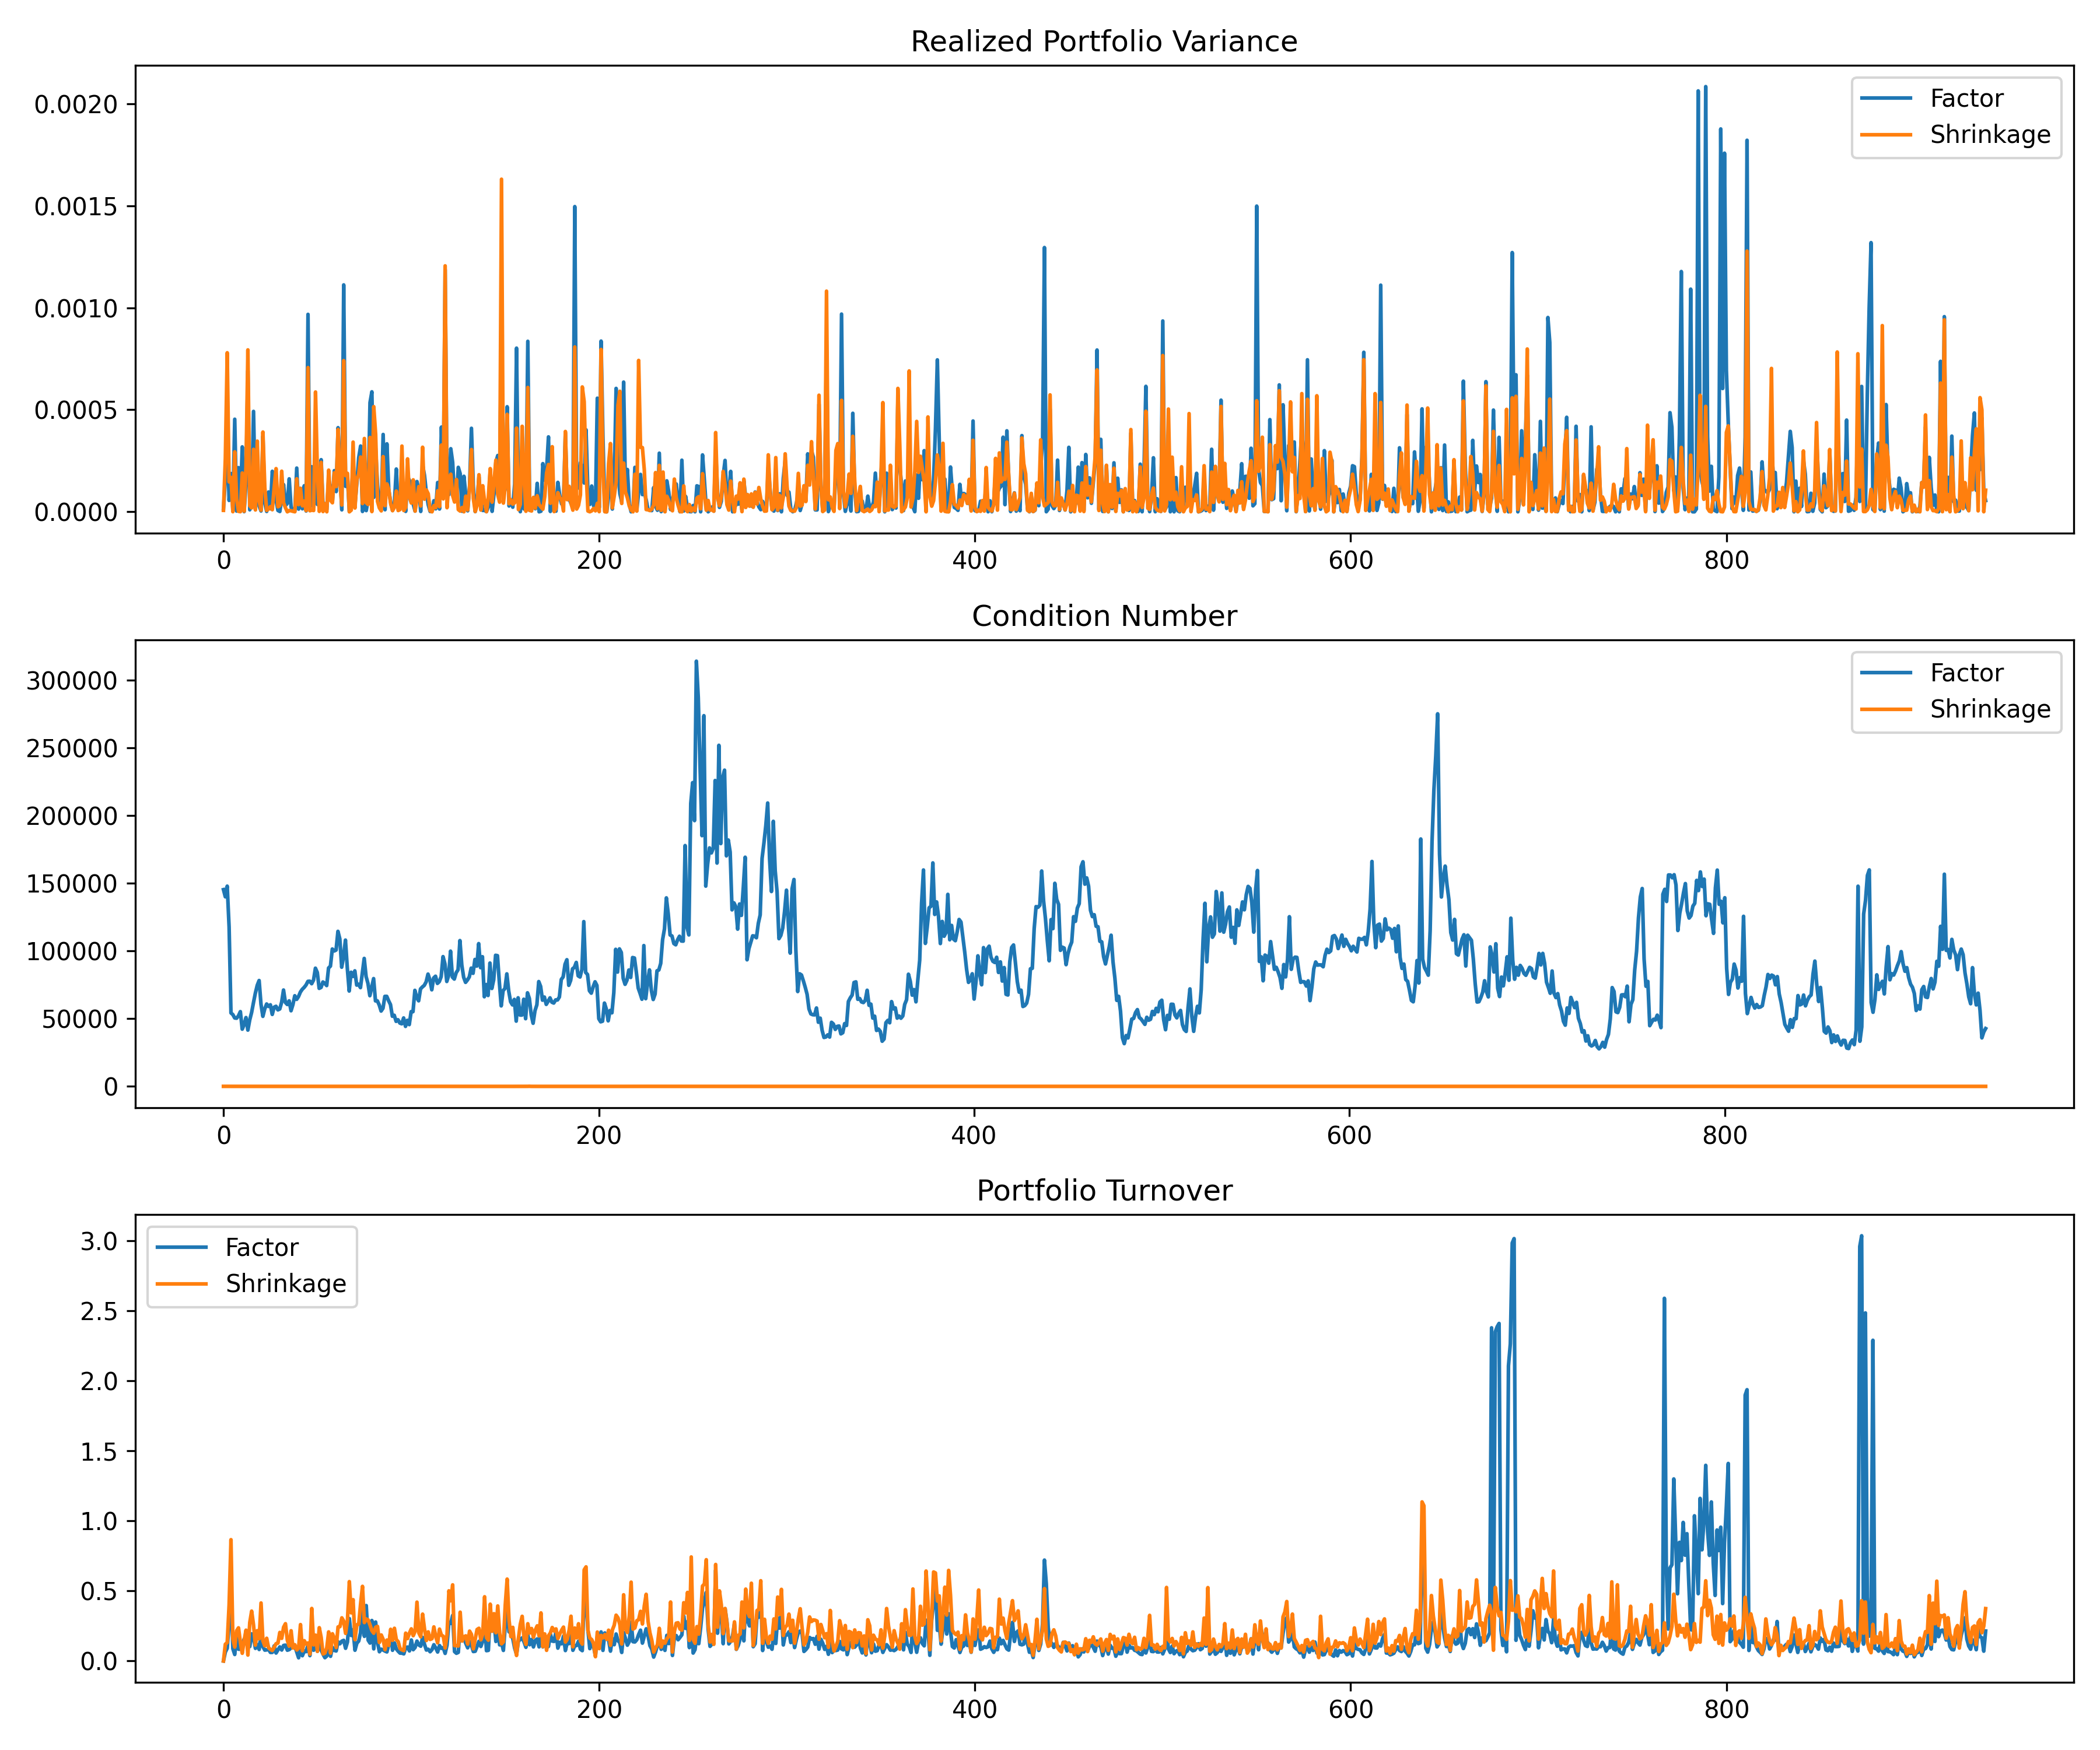
\includegraphics[width=\textwidth]{../input_files/plots/step_2_summary_plot_1775415610.png}
    \caption{Comparison of the factor-based and shrinkage covariance estimators across realized portfolio variance (top), covariance matrix condition number (middle), and portfolio turnover (bottom). The factor-based approach exhibits significant numerical instability, evidenced by a high and volatile condition number, which translates into higher realized portfolio variance compared to the robust shrinkage estimator. Despite this performance gap, both methods result in comparable levels of portfolio turnover, suggesting the rebalancing in the factor-based strategy is driven by estimation noise rather than signal.}
    \label{fig:summary_plot}
\end{figure*}

\subsection{Diagnosing the source of factor model instability}
To investigate the cause of the factor model's poor performance, we first assess whether the chosen factors adequately capture the systematic risk in the asset universe. The explanatory power of the two-factor model, as measured by the R-squared from the underlying OLS regressions, is shown in Figure \ref{fig:r_squared_plot}.

The explained variance ratio remains relatively stable over the 1,000-day period, fluctuating mostly between 0.4 and 0.6. The absence of a systematic decline or extreme volatility in the R-squared suggests that the two-factor structure provides a reasonably consistent explanation of the systematic components of asset returns. Therefore, the failure of the factor-based covariance estimator is unlikely to be caused by a fundamental lack of model span.

\begin{figure}[htbp]
    \centering
    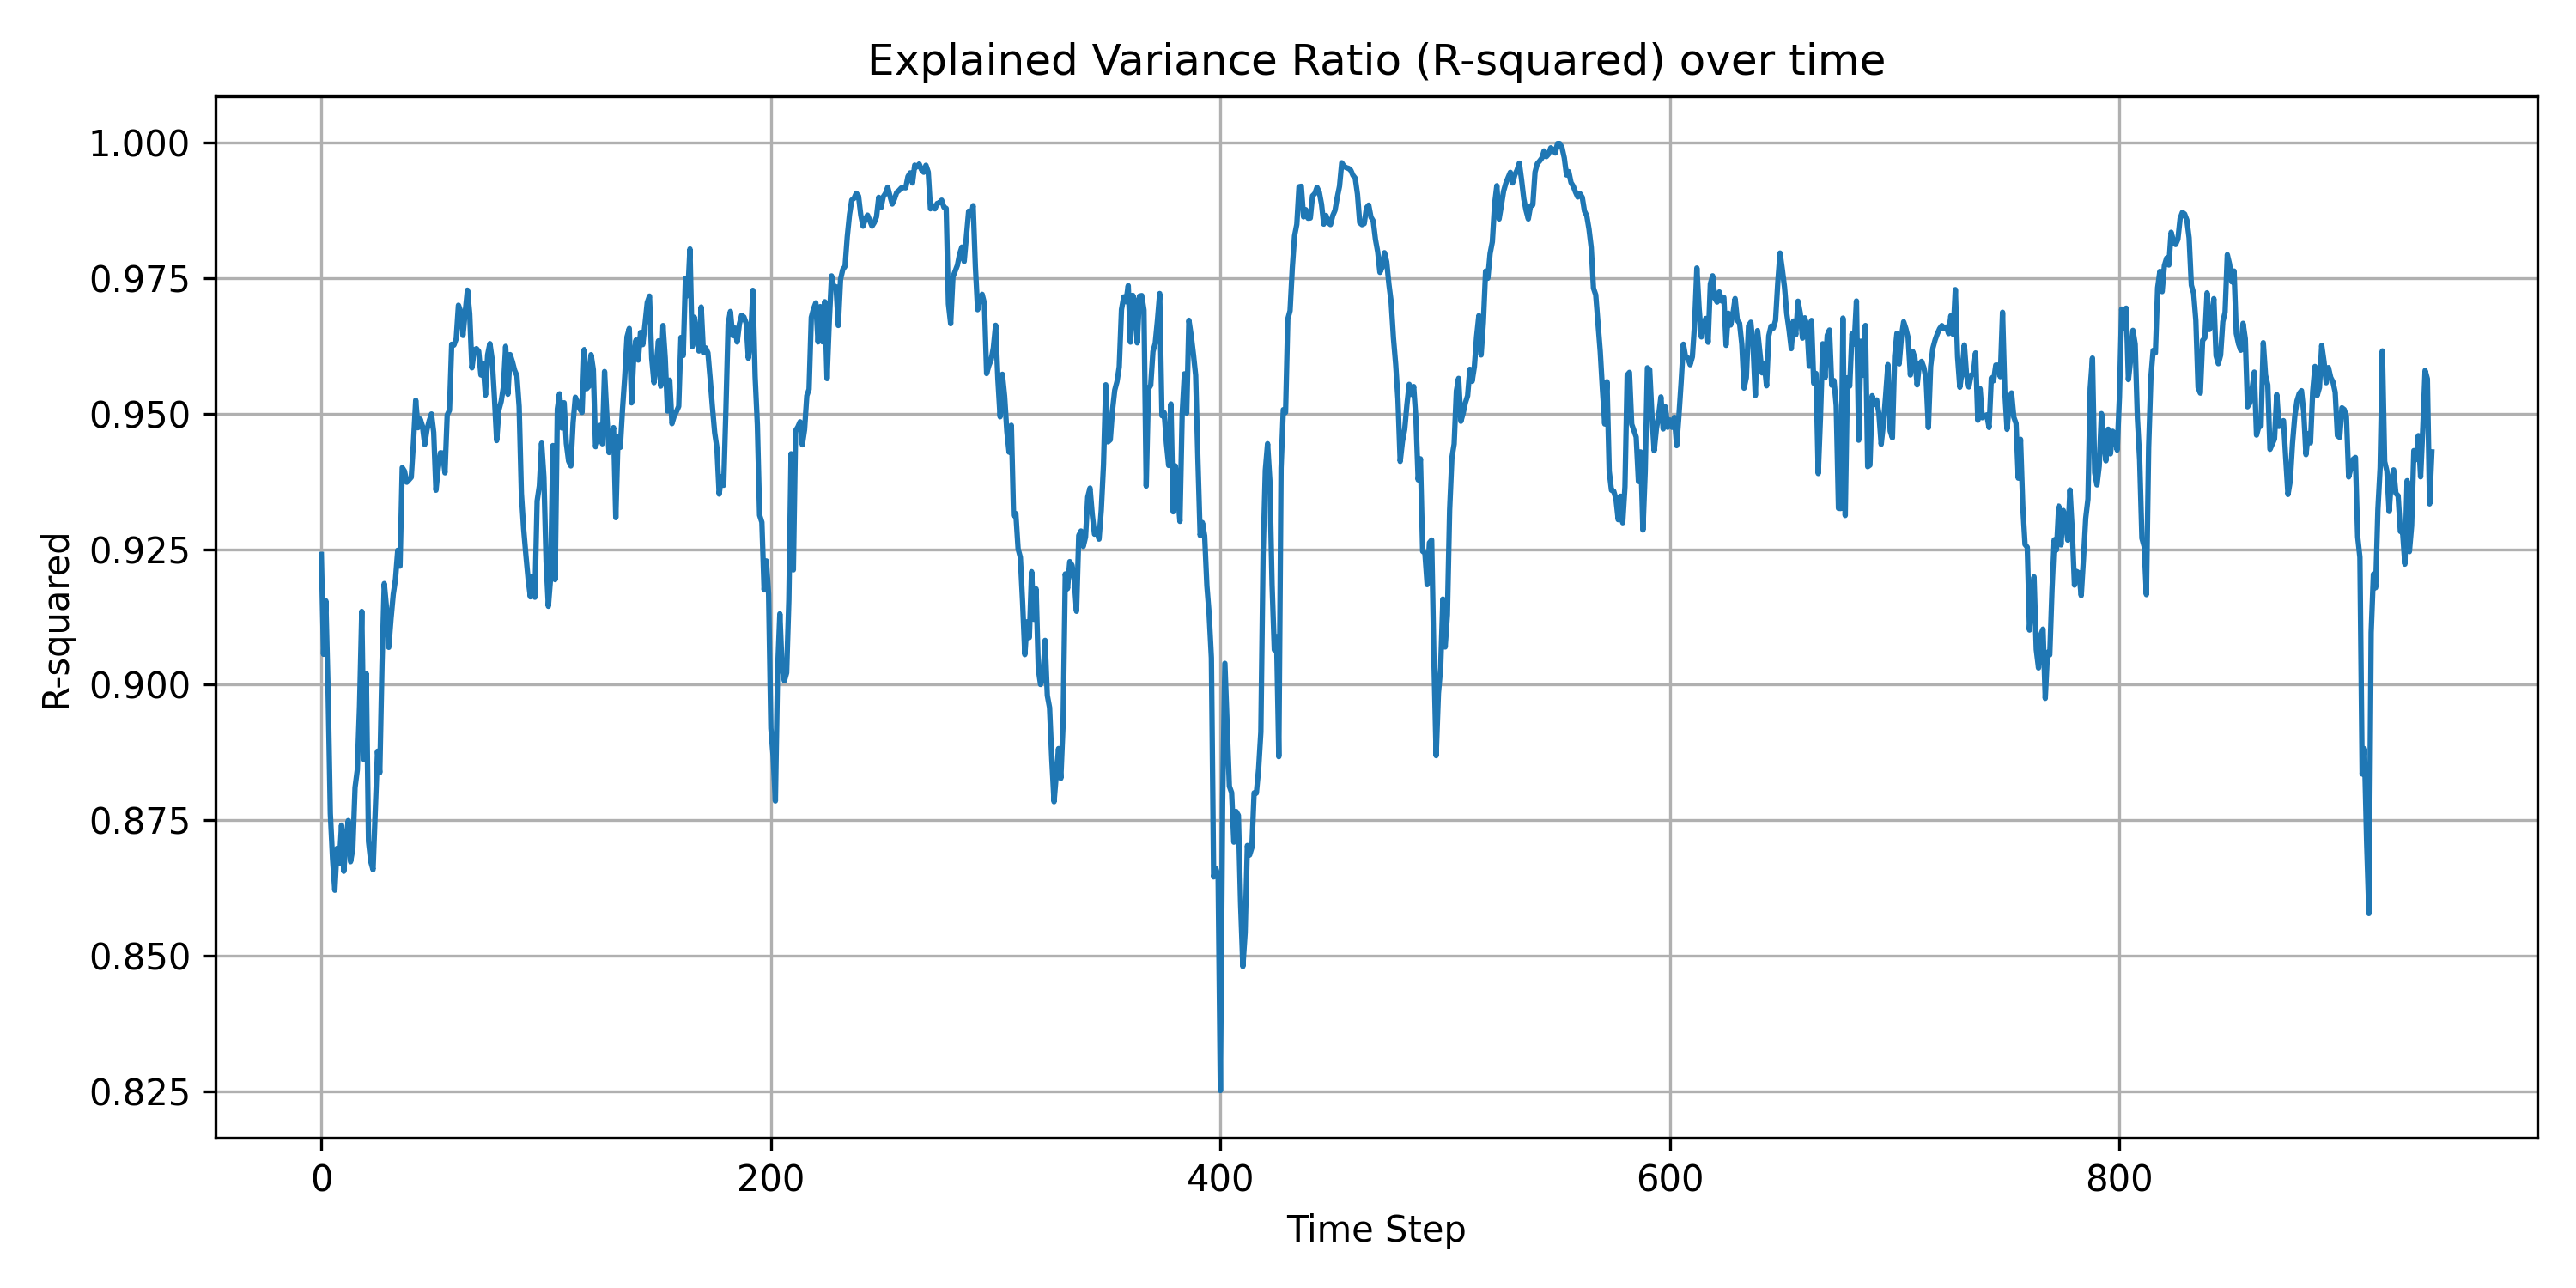
\includegraphics[width=\columnwidth]{../input_files/plots/step_2_r_squared_plot_1775415610.png}
    \caption{Explained Variance Ratio (R-squared) of the two-factor model over the 1,000-day simulation period. The relative stability of the R-squared indicates that the model span is sufficient to capture systematic returns, suggesting that the underperformance of the factor-based covariance estimator is not driven by a failure to explain systematic risk.}
    \label{fig:r_squared_plot}
\end{figure}

Instead, the evidence points toward the estimation of the idiosyncratic variance matrix, $\mathbf{\Psi}_t$, as the primary source of instability. The final covariance matrix is reconstructed by combining the systematic component with the idiosyncratic variances and then scaling by GARCH-forecasted volatilities. Any estimation error in the diagonal elements of $\mathbf{\Psi}_t$, which are derived from regression residuals over a short 60-day window, is amplified by the squared GARCH volatility forecasts ($\hat{\sigma}_{i,t}^2$). For assets with high and time-varying idiosyncratic risk, this process introduces significant noise into the final covariance matrix. This noise is the direct cause of the extremely high condition numbers observed in Figure \ref{fig:summary_plot}. The structural model, while theoretically sound, proves to be fragile in practice because it overfits to the noisy idiosyncratic component of returns---a problem that the regularization inherent in the shrinkage estimator is specifically designed to mitigate.

\section{Conclusions}
\label{sec:conclusions}
This paper addressed the challenge of estimating the covariance matrix of asset returns for Minimum Variance Portfolio optimization, particularly in an environment characterized by time-varying volatility and significant idiosyncratic risk. We conducted a direct empirical comparison of two dynamic estimation strategies: a structural two-factor model designed to isolate systematic risk, and a Ledoit-Wolf shrinkage estimator that regularizes the sample covariance matrix. The analysis was performed on a 1,000-day panel of ten large-cap equities, with both methods applied within a 60-day rolling window to returns that were first filtered through asset-specific GARCH(1,1) models to account for heteroskedasticity.

Our results demonstrated that the shrinkage-based approach consistently constructed portfolios with lower out-of-sample realized variance compared to the factor-based model. A diagnostic analysis of the estimated covariance matrices revealed the source of this performance gap. The factor-based covariance matrix was found to be severely ill-conditioned, exhibiting an extremely high and volatile condition number. In contrast, the shrinkage estimator produced a well-conditioned and numerically stable matrix throughout the backtest. This instability in the factor model indicates that its inverse, and therefore the resulting portfolio weights, were highly sensitive to small estimation errors.

We learned that the failure of the factor model was not caused by a lack of explanatory power, as the model's R-squared was reasonably stable, suggesting the factors adequately captured systematic risk. The primary source of instability was the estimation of the idiosyncratic variance components. Estimation errors in the idiosyncratic variances, derived from regression residuals over a short window, were significantly amplified when re-scaled by the GARCH volatility forecasts. This process of overfitting to noisy, asset-specific risk components compromised the stability of the entire covariance matrix. In conclusion, this study shows that while structural models provide an intuitive framework for risk, they can be fragile to the propagation of estimation error. In a dynamic and heteroskedastic environment, the statistical regularization provided by the shrinkage estimator proved to be a more robust and effective method for producing reliable covariance estimates for portfolio optimization.


\bibliography{bibliography}{}
\bibliographystyle{unsrt}

\end{document}
